% "{'classe':('PSI'),'chapitre':'slci_correcteur','type':('colle'),'titre':'Asservissement en température d\\'un four', 'source':'Équipe PT La Martinière Monplaisir','comp':('C1-02','C2-04'),'corrige':False}"
%\setchapterimage{bandeau}
\chapter*{Colle \arabic{cptColle} \\ 
Asservissement en température d'un four -- 
\ifprof Corrigé \else Sujet \fi}
\addcontentsline{toc}{section}{Colle \arabic{cptColle} :
Asservissement en température d'un four -- 
\ifprof Corrigé \else Sujet \fi}

\iflivret \stepcounter{cptColle} \else
\ifprof  \stepcounter{cptColle} \else \fi
\fi

\setcounter{question}{0}
\marginnote{Équipe PT -- La Martinière Monplaisir.}
\marginnote[1cm]{
\UPSTIcompetence[2]{C1-02}
\UPSTIcompetence[2]{C2-04}}


%\begin{marginfigure} [4cm]
%\includegraphics[width=\linewidth]{fig_01a}
%\end{marginfigure}





Un four électrique destiné au traitement thermique d'objets est constitué d'une enceinte close chauffée par une résistance électrique alimentée par une tension v(t). Dix objets peuvent prendre place simultanément dans le four. Le traitement thermique consiste à maintenir les objets pendant 1 heure à une température de 1200\degres C (régulée de façon optimale car les objets sont détruits si la température dépasse  1400\degres C).
Entre deux cuissons, un temps de 24 minutes est nécessaire pour procéder au refroidissement du four et à la manutention.
Le four est régi par l’équation différentielle : $\dfrac{\text{d}\theta(t)}{\text{d}t}+2000\dfrac{\text{d}^2\theta(t)}{\text{d}t^2}=0,02 v(t)$.


\question{Calculer la fonction de transfert $G(p)$ du four en boucle ouverte. Quel est le gain statique du four? Que se passerait-il si on alimentait le four en continu et en boucle ouverte ?}

On décide de réguler la température $\theta(t)$ dans le four en utilisant un capteur de température qui délivre une tension $u(t)$. Le capteur est régi par l’équation différentielle :  $u(t)+2\dfrac{\text{d}u(t)}{\text{d}t}=5\cdot 10^{-3} \theta(t)$. On introduit également un gain $K$ dans la chaîne directe.

\question{Faire le schéma de la boucle de régulation et calculer sa fonction de transfert en boucle fermée. Rappeler  les conditions de stabilité d'un système.}


On donne $t_m$ le temps de montée du système en BF : $t_m\simeq \dfrac{3}{\omega_{\text{co}}}$ avec $\omega_{\text{co}}$ est la pulsation de coupure à \SI{0}{dB} du système en BO.  


\question{On souhaite se placer dans des conditions de stabilité suffisantes en imposant une marge de phase $\Delta \varphi= 45\degres$. Quelle  est dans ces conditions, la valeur du temps de montée en boucle fermée ?}

On souhaite atteindre une cadence de 100 pièces en 24h, ceci est obtenu pour $K=11,3$.

\question{Pour conserver une marge de phase égale à 60° on introduit une correcteur à avance de phase sous la forme $C(p)=K_a \dfrac{1+aTp}{1+Tp}$. Déterminer les constantes du correcteur.}


\ifprof
\begin{center}
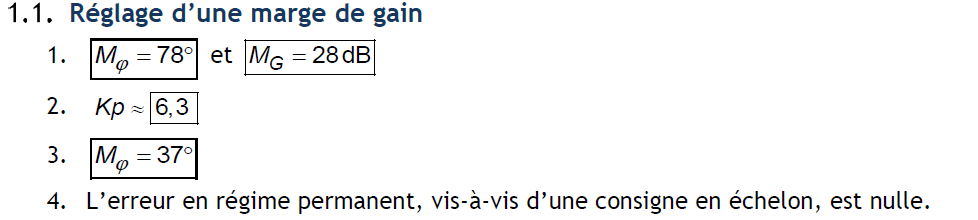
\includegraphics[width=\linewidth]{cor_01}
\end{center}
\else
\fi
